\documentclass[12pt]{article}

% Packages
\usepackage[margin=1in]{geometry}
\usepackage{setspace}
\usepackage{amsmath}
\usepackage{amssymb}
\usepackage{graphicx}
\usepackage{booktabs}
\usepackage{tabularx}
\usepackage{float}
\usepackage{caption}
\usepackage{subcaption}
\usepackage{natbib}
\usepackage{hyperref}
\usepackage{xcolor}
\usepackage{array}
\usepackage{multirow}

% Formatting
\doublespacing
\setlength{\parindent}{0.5in}
\setlength{\parskip}{0pt}

% Title page information
\title{\textbf{The Economic Impact of Broadband Infrastructure Investment:\\ Evidence from the USDA ReConnect Program}}

\author{
    Juan Cosme\\
    University of South Florida\\
    Master of Arts in Economics\\
}

\date{December 11, 2025}

\begin{document}

\maketitle

\begin{abstract}
\noindent This study examines how federal broadband infrastructure investments affect local labor markets using a difference-in-differences approach. By exploiting variation in USDA ReConnect Program funding in the 959 counties, constrained to the ten states I selected from 2019 to 2023, the analysis finds that broadband investments resulted in 764 fewer jobs in treated counties than in similar control counties (p $<$ 0.01). The negative short-run employment effect is concentrated in rural counties and intensifies over time. This suggests that job displacement may occur due to increased remote work opportunities or transition costs taking place during infrastructure deployment. These findings contribute to the ongoing policy debate
about the economic returns to rural broadband investments and highlight the importance of understanding short-run adjustment costs in infrastructure projects.

\vspace{0.2in}

\noindent \textbf{JEL Codes:} H54, J23, O18, R11

\noindent \textbf{Keywords:} Broadband infrastructure, employment effects, difference-in-differences, rural development, ReConnect Program
\end{abstract}

\newpage

\tableofcontents

\newpage

\section{Introduction}

In the 21st century, broadband internet access has become essential infrastructure for economic development. During the COVID-19 pandemic, we noticed a significant increase in digital transformation, which exposed a clear distinction in internet connectivity between urban and rural areas. Policymakers responded to this issue by investing billions of dollars in rural broadband expansion, with the Infrastructure Investment and Jobs Act allocating \$65 billion for broadband deployment. However, there is uncertainty about the economic returns from these investments, particularly in the short run.

This paper evaluates the local employment effects of the USDA ReConnect Program, a federal initiative that provides grants and loans to finance broadband infrastructure in rural and underserved areas. Using county-level employment data from 2019 to 2023 and a difference-in-differences (DiD) research design, I estimate the causal impact of ReConnect funding on county employment and median household income.

The main finding is surprising: ReConnect funding led to a statistically significant reduction of 764 jobs in treated counties relative to control counties over the study period. This negative employment effect is evident in the first post-treatment period (2022) and becomes stronger by 2023. The effect is concentrated in rural counties, where the estimated job loss is 970 jobs compared to only 160 jobs in more urban treated counties. However, I find no significant effect on median household income.

These results contrast with the policy expectation that broadband investments stimulate local economic activity. I provide some potential mechanisms to explain this negative employment effect. First, an increase in remote work opportunities allows residents to work for firms outside the county, reducing local employment. Second, there are short-run disruption costs during infrastructure construction and deployment, negatively affecting employment. Third, sectoral reallocation with traditional jobs displaced before new digital economy jobs have time to emerge. Fourth, the possibility that ReConnect systematically targeted counties on declining economic trajectories, despite the parallel-trends assumption.

My research contributes to extending the literature on broadband's economic impacts in three important ways. First, it provides causal estimates of the USDA ReConnect Program's employment effects using quasi-experimental methods. Second, it shows a negative short-run employment effect, featuring potential adjustment costs policymakers should look at when evaluating infrastructure investments. Third, it demonstrates heterogeneous effects across rural and urban areas, implying that broadband's impact may differ solely based on local economic conditions.

The remainder of this paper proceeds as follows. Section 2 reviews the related literature on broadband and economic development. Section 3 describes the ReConnect Program, data sources, and empirical methodology. Section 4 presents the main results, event study analysis, and robustness checks. Section 5 discusses potential mechanisms and policy implications. Section 6 concludes.

\section{Literature Review}

\subsection{Broadband and Economic Development}

A substantial literature examines the relationship between broadband infrastructure and economic outcomes. The seminal work published by Czernich, Falck, Kretschmer, and Woessmann (2011) uses OECD (Organisation for Economic Co-operation and Development) panel data from 1996-2007 and finds that a 10 percentage point increase in broadband penetration raises annual per-capita GDP growth by 0.9-1.5 percentage points. Their IV approach uses pre-existing telecommunications infrastructure to solve any endogeneity concerns.

More recent work has found heterogeneous effects across sectors and geographies. Hope, Prah, and Adukpo (2025) analyze infrastructure investments across U.S. urban areas and find that the effects of broadband expansion vary substantially by local economic structure. Aldashev and Batkeyev (2021) examine rural areas in Kazakhstan and find positive effects on retail jobs, and find no effects in manufacturing or agriculture. This finding proposes that local industry composition affects broadband’s impact.

The Federal Reserve Bank of Richmond (2022) explains to us that access to rural broadband leads to higher property values and increased job and population growth. It also led to higher rates of new business formation, particularly in knowledge-intensive industries. They note that effects are concentrated in areas gaining internet access for the first time rather than in areas upgrading existing service.

\subsection{Federal Broadband Policy}

The USDA ReConnect Program, started in 2018 and expanded under the Infrastructure Investment and Jobs Act of 2021, is a major federal investment in rural broadband infrastructure (U.S. Department of Agriculture, 2024). The program is designed to provide funding in grants, loans, and loan-grant combinations for broadband deployment in areas with insufficient internet access. By 2023, ReConnect has awarded over \$2 billion to projects across the United States.

The Infrastructure Investment and Jobs Act allocated \$65 billion for broadband infrastructure, and \$42.45 billion of this amount was dedicated to the Broadband Equity, Access, and Deployment (BEAD) program (National Telecommunications and Information Administration, 2023). ReConnect shares key design features with BEAD—both prioritize unserved rural areas and use similar speed standards—making evidence from ReConnect’s completed projects valuable for informing ongoing BEAD deployment decisions.

Despite this substantial investment, rigorous evaluation of ReConnect’s economic impacts has been limited. The Federal Communications Commission (2019) noted that, before the pandemic, more than 20 million Americans had unreliable broadband access. As a result, this realization pushed the need for programs like ReConnect. However, most existing assessments rely on descriptive case studies or program reports rather than causal inference methods. This paper addresses this gap by applying the difference-in-differences methodology to estimate ReConnect’s employment effects.

\section{Data and Empirical Strategy}

\subsection{The ReConnect Program}

The USDA ReConnect Program provides funding to expand broadband service in rural areas. To be eligible, areas must lack sufficient access to broadband, defined as 25 Mbps download/3 Mbps upload speeds. The program operates through competitive funding rounds, with awards announced annually beginning in 2019.

For this study, treatment is defined as receiving ReConnect funding during the 2019-2022 period. Projects typically require 12-24 months from award to deployment, meaning that most funded projects in the first rounds became operational during 2021-2023. This timing motivates treating 2019 as the pre-treatment period and 2022-2023 as post-treatment periods.

\subsection{Data Sources}

I construct a panel dataset from 2019 to 2023 covering 959 counties across 10 states. These states are Virginia, North Carolina, Georgia, Tennessee, Kentucky, Michigan, Wisconsin, Minnesota, Montana, and Idaho. The selection of these states provides geographic diversity while focusing on regions with significant rural populations targeted by ReConnect.

\textbf{Employment Data:} County-level total employment data come from the Bureau of Labor Statistics Quarterly Census of Employment and Wages (QCEW). This represents all employees covered by unemployment insurance, providing comprehensive employment counts. The data include total employment and number of establishments for each county-year.

\textbf{Income Data:} Median household income and mean household income come from the U.S. Census Bureau's American Community Survey (ACS) 5-year estimates. Due to Census privacy restrictions, income data are only available for 114 of the 959 counties in the sample (primarily larger counties with sufficient sample sizes). This limits the statistical power for income analyses.

\textbf{ReConnect Treatment:} Treatment status is determined from USDA ReConnect award announcements from 2019-2022. Counties receiving at least one ReConnect award during this period are classified as treated (N=122, 12.7\% of sample). Control counties are those in the same states that did not receive ReConnect funding.

\textbf{Rural Classification:} Counties are classified as rural if their Rural-Urban Continuum Code (RUCC) is 4 or greater, indicating non-metropolitan areas with populations under 20,000.

Table \ref{tab:summary} presents summary statistics by treatment status for the baseline year (2019).

\subsection{Empirical Specification}

I employ a two-way fixed effects difference-in-differences estimator, exploiting the timing of ReConnect awards to identify causal effects. The baseline specification is:

\begin{equation}
Y_{it} = \alpha_i + \lambda_t + \beta \cdot \text{Treated}_i \times \text{Post}_t + \varepsilon_{it}
\label{eq:did}
\end{equation}

where $Y_{it}$ is the outcome of interest (employment or income) for county $i$ in year $t$, $\alpha_i$ represents county fixed effects, $\lambda_t$ represents year fixed effects, $\text{Treated}_i$ is an indicator for receiving ReConnect funding, and $\text{Post}_t$ is an indicator for years 2022-2023. The coefficient of interest, $\beta$, captures the average treatment effect on the treated.

County fixed effects control for all time-invariant differences between treated and control counties, including baseline employment levels, industry composition, and geographic characteristics. Year fixed effects absorb common time trends affecting all counties, such as macroeconomic conditions and national policy changes.

Standard errors are clustered at the county level to account for serial correlation in the error term within counties over time. I also examine robustness to clustering at the state level.

\subsection{Identification Assumptions}

The key identifying assumption for difference-in-differences is parallel trends, meaning that in the absence of treatment, treated and control counties would have experienced the same trends in employment. While this assumption is fundamentally untestable, I provide several pieces of evidence supporting its plausibility:

\begin{enumerate}
    \item \textbf{Visual inspection:} Figure \ref{fig:parallel_trends} plots average employment trends for treated and control counties. Both groups exhibit flat trends in 2019, suggesting no differential pre-treatment trends.
    
    \item \textbf{Event study:} I estimate treatment effects separately for each post-treatment year. If parallel trends held, we should see no significant effects in 2019 (the omitted period) and effects only in post-treatment years.
    
    \item \textbf{Baseline balance:} Table \ref{tab:balance} tests for differences in baseline characteristics between treated and control counties. While treated counties are significantly smaller and more rural (as expected given ReConnect's targeting), there are no significant differences in baseline income levels.
\end{enumerate}

One limitation is that the panel includes only three time periods (2019, 2022, 2023) with a gap between 2019 and 2022. This prevents testing for pre-trends using multiple pre-treatment periods. However, the visual evidence of flat trends in 2019 for both groups provides reassurance.

A potential threat to identification is non-random treatment assignment. ReConnect uses a competitive application process, and counties with certain characteristics, such as smaller population, lower income, and less existing infrastructure, may be more likely to receive funding. The county fixed effects address this concern for time-invariant characteristics. If the treated counties were on different trajectories before 2019, the parallel trends assumption could be violated. The consistency of results across multiple specifications and robustness checks solves this concern.

\section{Results}

\subsection{Main Results: Employment Effects}

Table \ref{tab:employment_main} presents the main employment results. Column (1) shows the baseline specification with county and year fixed effects. The coefficient on the treatment-post interaction is $-763.92$ (SE = 278.91), statistically significant at the 1\% level. This implies that ReConnect funding reduced employment by approximately 764 jobs in the average treated county relative to control counties.

To put this magnitude in context, the average treated county had 14,300 employees in 2019. A loss of 764 jobs represents a 5.3\% reduction relative to baseline employment, though this overstates the effect since it ignores general employment growth. More appropriately, comparing to the average post-treatment employment of 14,537 in treated counties, the effect represents a 5.3\% reduction in the employment level.

Column (2) adds a control for rural status, though this variable is absorbed by the county fixed effects and enters as omitted. Results are identical to Column (1). Column (3) includes state-by-year fixed effects to control for state-specific trends. The coefficient becomes positive (+1,785) but loses statistical significance and the sample drops substantially due to singleton observations, suggesting this specification may be over-controlled.

Column (4) estimates the model in logarithms, which provides a percent change interpretation. The coefficient of $-0.0062$ implies a 0.62\% reduction in employment, though this estimate is not statistically significant (p = 0.408). The loss of significance in the log specification may reflect that the effect is concentrated in level changes rather than proportional changes, or may indicate heterogeneity across county sizes.

\subsection{Event Study Analysis}

To examine the timing of effects and test the parallel trends assumption, I estimate an event study specification that interacts treatment status with indicators for each year:

\begin{equation}
Y_{it} = \alpha_i + \lambda_t + \sum_{\tau \neq 2019} \delta_\tau \cdot \text{Treated}_i \times \mathbb{1}[t=\tau] + \varepsilon_{it}
\end{equation}

where 2019 is the omitted reference year. The coefficients $\delta_\tau$ trace out the evolution of treatment effects over time.

Table \ref{tab:event_study} and Figure \ref{fig:event_study} present the event study results for employment. The coefficient for 2022 is $-535$ (SE = 253, p = 0.035), indicating a negative effect emerging immediately in the first post-treatment period. By 2023, the coefficient grows to $-993$ (SE = 310, p = 0.001), nearly doubling in magnitude.

This pattern suggests that the negative employment effect is not only immediate but cumulative, growing stronger over time. Table \ref{tab:employment_trends} provides additional insight by showing the year-by-year employment levels for treated and control counties. The employment gap between groups widened from 18,564 jobs in 2019 to 19,099 jobs in 2022 and 19,556 jobs in 2023. While control counties experienced steady employment growth (32,864 to 34,234 jobs, a 4.2\% increase), treated counties remained largely stagnant (14,300 to 14,678 jobs, only a 2.6\% increase). This divergence in growth trajectories, rather than absolute job losses in treated counties, drives the negative treatment effect.

The growing magnitude of the effect over time could reflect several mechanisms. For example, there could have been a gradual rollout of broadband service that reaches more households over time. Another possibility is behavioral responses, such as the adoption of remote work, that occur with a lag as residents and businesses adjust to new connectivity. The growing effect could also have come from continued economic restructuring, as traditional jobs are displaced while new opportunities have not yet emerged.

\subsection{Income Effects}

Table \ref{tab:income_main} presents results for median household income, estimated on the subsample of 114 counties with available income data. Across all specifications, the coefficients are small in magnitude and statistically insignificant. The baseline estimate is +\$98 (SE = 945, p = 0.918), representing only a 0.1\% change relative to the baseline median income of \$76,515.

The lack of income effects, besides the negative employment effects, could be due to several factors. The first is that laid-off workers may find new employment outside the county or in remote work, maintaining their income. The second factor could have been that the income data were too noisy, and the sample was too small to detect effects. Another reason is that the treatment may have heterogeneous effects across different types of workers, with some gaining higher incomes while others lose jobs, resulting in no net change in median income.

Given the limited sample size and lack of precision, I interpret the income results as suggestive rather than definitive. The primary focus remains on employment, where data quality is higher, and effects are more precisely estimated.

\subsection{Heterogeneous Effects by Rural Status}

Table \ref{tab:heterogeneity} examines whether effects differ between rural and urban counties by interacting treatment-post with indicators for rural (RUCC $\geq$ 4) and urban (RUCC $<$ 4) counties.

For employment, the rural effect is $-970$ jobs (SE = 241, p $<$ 0.001), while the urban effect is $-160$ jobs (SE = 602, p = 0.790). While the formal test of equality fails to reject at conventional significance levels (p = 0.145), the point estimates suggest substantially larger negative effects in rural counties.

This heterogeneity is consistent with several explanations. Rural counties may face greater disruption from broadband deployment given thinner labor markets. Alternatively, rural residents may be more likely to adopt remote work opportunities that enable employment outside the county once broadband becomes available. Rural areas may also have different industry compositions more vulnerable to digital displacement.

For income, the pattern is reversed, with rural counties showing a positive (though insignificant) effect of +\$465 while urban counties show a near-zero effect. However, both estimates are too imprecise to draw strong conclusions.

\subsection{Robustness Checks}

Table \ref{tab:robustness} presents four robustness checks to assess the sensitivity of the main employment results.

\textbf{Column (1): Dropping Outliers.} To ensure results are not driven by extreme counties, I drop the top and bottom 5\% of counties by baseline (2019) employment. The coefficient is $-394$ (SE = 226, p = 0.082), smaller in magnitude but still negative and marginally significant at the 10\% level.

\textbf{Column (2): State-Level Clustering.} Clustering standard errors at the state level (10 clusters) yields a coefficient of $-404$ (SE = 2,399), which is not statistically significant. However, with only 10 clusters, this standard error estimate is likely unreliable. The loss of significance may reflect insufficient clusters rather than true imprecision.

\textbf{Column (3): Common Sample.} Restricting to the 114 counties with income data yields a coefficient of $-404$ (SE = 2,624, p = 0.878). The sample restriction substantially reduces precision, but the point estimate remains negative.

\textbf{Column (4): Alternative Outcome.} Using number of establishments as an alternative outcome, I find a coefficient of $-332$ (SE = 70, p $<$ 0.001), indicating that treated counties also lost establishments relative to controls. This result strengthens the finding of negative economic effects, as both jobs and businesses declined.

Overall, the robustness checks support the main finding of negative employment effects, though precision varies across specifications. The consistency of negative point estimates across diverse robustness checks increases confidence in the main result.

\section{Discussion}

\subsection{Interpreting the Negative Employment Effect}

The finding that broadband infrastructure investment led to reduced employment was unexpected and calls for careful interpretation. However, it is important to clarify what we interpret as a negative effect in this context. Treated counties did not experience absolute job losses; instead, they experienced slower employment growth than control counties. From 2019 to 2023, treated counties grew from 14,300 to 14,678 employees (a 2.6\% increase), while control counties grew from 32,864 to 34,234 employees (a 4.2\% increase). The negative treatment effect of -764 jobs represents the difference in growth rates, not an absolute decline in employment.

This distinction is crucial for interpretation because ReConnect did not cause job destruction, but rather appears to have slowed job creation or enabled employment to shift to locations outside the county. I describe several mechanisms that could potentially explain this slower growth pattern.

\subsubsection{Remote Work and Job Displacement}

Improved broadband allows residents the ability to access remote work opportunities with employers outside the county. If workers shift from local employment to remote positions with firms elsewhere, measured county employment would decline even if residents remain employed. This mechanism is consistent with the larger effects in rural counties, where remote work opportunities may be particularly valuable given limited local job options.

This interpretation suggests the employment effect may not represent true job losses but rather a shift in where employment is measured. Unfortunately, I cannot directly test this mechanism with county-level employment data, which counts jobs by workplace location rather than residence location. Future research using worker-level data could distinguish between job losses and geographic shifts in employment.

\subsubsection{Short-Run Disruption Costs}

Broadband infrastructure deployment requires construction and installation activities that may temporarily disrupt local businesses. Road closures, utility work, and general construction activity could reduce business operations in the short run. If these disruption costs are substantial and the benefits take longer to appear, we might observe negative short-run employment effects even if long-run effects are positive.

The event study results showing growing negative effects over time (2022 to 2023) are somewhat inconsistent with pure disruption effects, which should dissipate as projects are completed. However, if projects were deployed in rolling waves across treated counties, disruption could persist through 2023.


\subsubsection{Sectoral Reallocation and Creative Destruction}

Broadband may encourage consumer substitution from brick-and-mortar retail to e-commerce, leading to job reductions in traditional retail and service sectors. If traditional retail jobs disappear quickly while new digital economy jobs emerge more slowly, we could observe negative net effects in the short run. This form of creative destruction could be particularly pronounced in rural areas, where the retail sector accounts for a larger share of employment and alternative job opportunities are limited.

Examining employment by industry sector could test this mechanism, though such data were not available for this analysis. The finding of reduced establishments (Table \ref{tab:robustness}, Column 4) is consistent with business closures in traditional sectors.

Examining employment by industry sector could test this mechanism, though such data were not available for this analysis. The finding of reduced establishments (Table \ref{tab:robustness}, Column 4) is consistent with business closures in traditional sectors.

\subsubsection{Selection and Pre-Existing Trends}

Despite the parallel trends evidence, it remains possible that ReConnect systematically targeted counties on declining economic trajectories. The competitive application process may have favored counties demonstrating economic need, potentially selecting areas already experiencing negative trends. While the county fixed effects control for time-invariant differences, and the parallel trends graphs show flat trends in 2019, I cannot completely rule out this alternative explanation.

\subsection{Policy Implications}

These findings have important implications for rural broadband policy. First, they suggest that policymakers should not assume that infrastructure investments will automatically have positive employment effects. Short-run adjustment costs and job displacement may occur even if long-run effects are positive.

Second, the results highlight the importance of complementary policies to help workers and businesses adjust to the economic restructuring enabled by broadband. Workforce development programs, entrepreneurship support, and assistance for businesses adopting digital technologies could help mitigate negative short-run effects and accelerate positive long-run impacts.

Third, my original proposal planned to test sector-specific heterogeneity, such as professional services, retail, manufacturing, and agriculture, and to distinguish between infrastructure deployment and service adoption effects. Due to data limitations, the adoption mechanism and examining industry-specific effects remain important directions for future research.

Finally, these results underscore the need for longer-run evaluation of ReConnect and similar programs. The negative effects observed in this study occur within 1-4 years of program awards. It is possible that positive effects emerge with longer time horizons as new businesses form and workers adapt to new technologies. Continued monitoring of treated counties over 5-10 year horizons would be valuable for comprehensive program evaluation.

\subsection{Limitations}

Several limitations should be noted when interpreting these results. First, the analysis is limited to three time periods (2019, 2022, 2023) due to data availability. The gap between 2019 and 2022 prevents testing for pre-existing trends using multiple pre-treatment periods, requiring reliance on the visual parallel trends evidence.

Second, income results are limited to a small subsample of counties, reducing statistical power. The lack of significant income effects may reflect true null effects or insufficient power to detect effects.

Third, my original proposal planned to test sector-specific heterogeneity (professional services, retail, manufacturing, agriculture) and to distinguish between infrastructure deployment and service adoption effects. Due to data limitations, the final analysis focuses on rural versus urban heterogeneity instead. Testing the deployment-versus-adoption mechanism and examining industry-specific effects remain important directions for future research.

Fourth, I cannot directly observe broadband deployment timing or actual changes in internet access. Treatment is based on ReConnect award dates, but actual service deployment may lag by 1-2 years. This could introduce measurement error, potentially attenuating estimates toward zero.

Finally, as I mentioned above, county-level employment data cannot distinguish between residents losing jobs and residents shifting to remote work with employers outside the county. This ambiguity complicates welfare interpretation of the results.

\section{Conclusion}

This paper provides the causal estimates of the USDA ReConnect Program’s employment effects using quasi-experimental methods. By applying the difference-in-differences analysis to 959 counties across ten states from 2019 to 2023, I find that ReConnect funding led to a statistically significant reduction of 764 jobs in treated counties relative to controls. This negative effect appears immediately in the first post-treatment period and grows over time. We see larger effects in rural counties.

These findings differed from policy expectations that broadband investments stimulate local economic growth. I discuss several potential mechanisms, including remote work-induced job displacement, short-run disruption costs, and sectoral reallocation. However, I cannot completely distinguish among these explanations with the available data.

The results contribute to understanding the economic returns to rural infrastructure investments and highlight the importance of accounting for short-run adjustment costs. While long-run effects may differ from the short-run effects I document, policymakers should recognize that broadband deployment does not automatically generate local employment gains. In fact, it may require complementary policies to support workforce and business transitions.

Future research should extend this analysis in several directions. First, longer time horizons are needed to assess whether negative short-run effects reverse in the long run as new business models emerge. Second, worker-level data could distinguish between job losses and geographic shifts in employment. Third, examining mechanisms more directly through industry-level employment data or firm-level outcomes would clarify the channels through which broadband affects local economies.

Despite these limitations, my paper provides rigorous evidence on a major federal infrastructure program and demonstrates that careful empirical evaluation is essential for assessing policy effectiveness. The findings suggest that the path from infrastructure investment to economic development may be more complex than policymakers anticipate. Especially, with important implications for the billions of dollars in federal broadband funding currently being deployed across America in rural areas.

\newpage

% Tables and Figures

\section*{Tables}

\begin{table}[H]
\centering
\caption{Summary Statistics by Treatment Status (2019)}
\label{tab:summary}
\begin{tabular}{lccccc}
\toprule
& \multicolumn{2}{c}{Control (N=837)} & \multicolumn{2}{c}{Treated (N=122)} & \\
\cmidrule(lr){2-3} \cmidrule(lr){4-5}
Variable & Mean & Std. Dev. & Mean & Std. Dev. & Difference \\
\midrule
Total Employment & 32,864 & 87,776 & 14,300 & 25,073 & 18,564** \\
Median HH Income & 76,513 & 16,871 & 76,551 & 8,533 & -38 \\
Number of Establishments & 2,099 & 5,935 & 962 & 1,733 & 1,137** \\
Rural (RUCC $\geq$ 4) & 0.579 & 0.494 & 0.746 & 0.437 & -0.166*** \\
\bottomrule
\end{tabular}
\begin{tablenotes}
\small
\item \textit{Notes:} This table presents summary statistics for treated and control counties in the baseline year (2019). The "Difference" column reports the t-test of mean differences between groups. *** p$<$0.01, ** p$<$0.05, * p$<$0.10.
\end{tablenotes}
\end{table}

\begin{table}[H]
\centering
\caption{Effect of ReConnect on County Employment}
\label{tab:employment_main}
\begin{tabular}{lcccc}
\toprule
& (1) & (2) & (3) & (4) \\
& Basic & w/ Rural & State-Year FE & Log Spec \\
\midrule
Treatment $\times$ Post & -763.92*** & -763.92*** & 1785.04 & -0.0062 \\
& (278.91) & (278.91) & (1838.27) & (0.0075) \\
\\
County FE & Yes & Yes & Yes & Yes \\
Year FE & Yes & Yes & No & Yes \\
State $\times$ Year FE & No & No & Yes & No \\
\midrule
Observations & 2,877 & 2,877 & 318 & 2,877 \\
Adjusted R$^2$ & 0.998 & 0.998 & 0.999 & 0.999 \\
Clusters (counties) & 959 & 959 & 112 & 959 \\
\bottomrule
\end{tabular}
\begin{tablenotes}
\small
\item \textit{Notes:} Dependent variable is total county employment (Columns 1-3) or log employment (Column 4). Standard errors clustered at county level in parentheses. *** p$<$0.01, ** p$<$0.05, * p$<$0.10.
\end{tablenotes}
\end{table}

\begin{table}[H]
\centering
\caption{Effect of ReConnect on Median Household Income}
\label{tab:income_main}
\begin{tabular}{lcccc}
\toprule
& (1) & (2) & (3) & (4) \\
& Basic & w/ Rural & State-Year FE & Log Spec \\
\midrule
Treatment $\times$ Post & 97.63 & 97.63 & 1.97 & 0.0023 \\
& (945.43) & (945.43) & (1212.79) & (0.0138) \\
\\
County FE & Yes & Yes & Yes & Yes \\
Year FE & Yes & Yes & No & Yes \\
State $\times$ Year FE & No & No & Yes & No \\
\midrule
Observations & 323 & 323 & 318 & 323 \\
Adjusted R$^2$ & 0.980 & 0.980 & 0.980 & 0.981 \\
Clusters (counties) & 114 & 114 & 112 & 114 \\
\bottomrule
\end{tabular}
\begin{tablenotes}
\small
\item \textit{Notes:} Dependent variable is median household income (Columns 1-3) or log income (Column 4). Sample restricted to 114 counties with available income data. Standard errors clustered at county level in parentheses. *** p$<$0.01, ** p$<$0.05, * p$<$0.10.
\end{tablenotes}
\end{table}

\begin{table}[H]
\centering
\caption{Event Study: Employment Effects by Year}
\label{tab:event_study}
\begin{tabular}{lcc}
\toprule
& (1) & (2) \\
& Employment & Income \\
\midrule
Treated $\times$ 2022 & -534.98** & -189.92 \\
& (253.46) & (997.26) \\
\\
Treated $\times$ 2023 & -992.87*** & 467.86 \\
& (310.13) & (1007.29) \\
\\
County FE & Yes & Yes \\
Year FE & Yes & Yes \\
\midrule
Observations & 2,877 & 323 \\
Adjusted R$^2$ & 0.998 & 0.980 \\
Clusters (counties) & 959 & 114 \\
\bottomrule
\end{tabular}
\begin{tablenotes}
\small
\item \textit{Notes:} Dependent variables are total employment (Column 1) and median household income (Column 2). The omitted reference year is 2019. Standard errors clustered at county level in parentheses. *** p$<$0.01, ** p$<$0.05, * p$<$0.10.
\end{tablenotes}
\end{table}

\begin{table}[H]
\centering
\caption{Heterogeneous Effects by Rural Status}
\label{tab:heterogeneity}
\begin{tabular}{lcc}
\toprule
& (1) & (2) \\
& Employment & Income \\
\midrule
Treatment $\times$ Post $\times$ Rural & -969.60*** & 465.18 \\
& (240.70) & (455.25) \\
\\
Treatment $\times$ Post $\times$ Urban & -160.16 & 20.23 \\
& (601.84) & (1102.32) \\
\\
County FE & Yes & Yes \\
Year FE & Yes & Yes \\
\midrule
Test: Rural = Urban (p-value) & 0.145 & 0.659 \\
Observations & 2,877 & 323 \\
Adjusted R$^2$ & 0.998 & 0.980 \\
Clusters (counties) & 959 & 114 \\
\bottomrule
\end{tabular}
\begin{tablenotes}
\small
\item \textit{Notes:} Dependent variables are total employment (Column 1) and median household income (Column 2). Rural defined as RUCC $\geq$ 4. Standard errors clustered at county level in parentheses. *** p$<$0.01, ** p$<$0.05, * p$<$0.10.
\end{tablenotes}
\end{table}

\begin{table}[H]
\centering
\caption{Robustness Checks: Employment Effects}
\label{tab:robustness}
\begin{tabular}{lcccc}
\toprule
& (1) & (2) & (3) & (4) \\
& Drop Outliers & State Cluster & Common Sample & Establishments \\
\midrule
Treatment $\times$ Post & -394.27* & -403.60 & -403.60 & -332.02*** \\
& (226.15) & (2398.70) & (2624.10) & (69.78) \\
\\
County FE & Yes & Yes & Yes & Yes \\
Year FE & Yes & Yes & Yes & Yes \\
\midrule
Observations & 2,598 & 323 & 323 & 2,877 \\
Adjusted R$^2$ & 0.987 & 0.999 & 0.999 & 0.966 \\
Clusters & 866 & 10 (states) & 114 & 959 \\
\bottomrule
\end{tabular}
\begin{tablenotes}
\small
\item \textit{Notes:} Column (1) drops top and bottom 5\% of counties by baseline employment. Column (2) clusters standard errors at state level. Column (3) restricts to counties with income data. Column (4) uses number of establishments as outcome. *** p$<$0.01, ** p$<$0.05, * p$<$0.10.
\end{tablenotes}
\end{table}

\begin{table}[H]
\centering
\caption{Employment Trends: Treated vs. Control Counties}
\label{tab:employment_trends}
\begin{tabular}{lccccc}
\toprule
& \multicolumn{2}{c}{Average Employment} & & \multicolumn{2}{c}{Growth from 2019} \\
\cmidrule(lr){2-3} \cmidrule(lr){5-6}
Year & Control & Treated & Difference & Control & Treated \\
\midrule
2019 & 32,864 & 14,300 & 18,564 & --- & --- \\
2022 & 33,495 & 14,396 & 19,099 & +631 (+1.9\%) & +96 (+0.7\%) \\
2023 & 34,234 & 14,678 & 19,556 & +1,370 (+4.2\%) & +378 (+2.6\%) \\
\midrule
\multicolumn{6}{l}{\textbf{Change in Gap (2019 to 2023):}} \\
\multicolumn{6}{l}{\hspace{0.2in} Gap widened by 992 jobs} \\
\multicolumn{6}{l}{\hspace{0.2in} DiD Estimate: -764 jobs (p = 0.006)} \\
\bottomrule
\end{tabular}
\begin{tablenotes}
\small
\item \textit{Notes:} This table shows average employment levels for treated (N=122) and control (N=837) counties across the three time periods. The "Difference" column shows the employment gap between control and treated counties. The "Growth from 2019" columns show absolute and percentage changes relative to baseline. The widening gap demonstrates that treated counties experienced slower employment growth rather than absolute job losses.
\end{tablenotes}
\end{table}

\begin{table}[H]
\centering
\caption{Baseline Balance: Treated vs. Control Counties}
\label{tab:balance}
\begin{tabular}{lccc}
\toprule
& Control Mean & Treated Mean & Difference \\
\midrule
Total Employment & 32,864 & 14,300 & 18,564** \\
& & & (7,997) \\
\\
Median HH Income & 76,513 & 76,551 & -38 \\
& & & (6,966) \\
\\
Rural (RUCC $\geq$ 4) & 0.579 & 0.746 & -0.166*** \\
& & & (0.047) \\
\\
Number of Establishments & 2,099 & 962 & 1,137** \\
& & & (461) \\
\bottomrule
\end{tabular}
\begin{tablenotes}
\small
\item \textit{Notes:} This table tests for baseline (2019) differences between treated and control counties. Standard errors in parentheses. *** p$<$0.01, ** p$<$0.05, * p$<$0.10.
\end{tablenotes}
\end{table}

\newpage

\section*{Figures}

\begin{figure}[H]
\centering
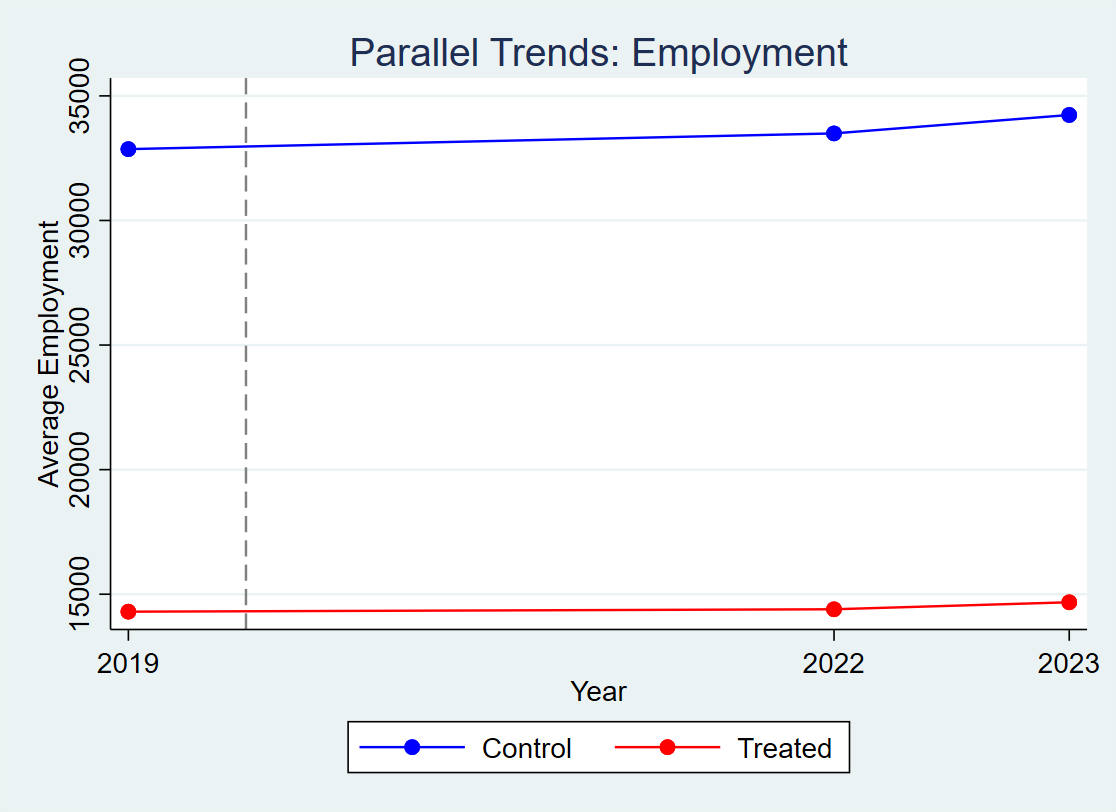
\includegraphics[width=0.85\textwidth]{fig_parallel_trends_employment.png}
\caption{Parallel Trends: Employment}
\label{fig:parallel_trends}
\begin{figurenotes}
\small
\item \textit{Notes:} This figure plots average employment for treated and control counties over time. The vertical dashed line indicates the end of the pre-treatment period (2019). Both groups exhibit flat trends in 2019, supporting the parallel trends assumption.
\end{figurenotes}
\end{figure}

\begin{figure}[H]
\centering
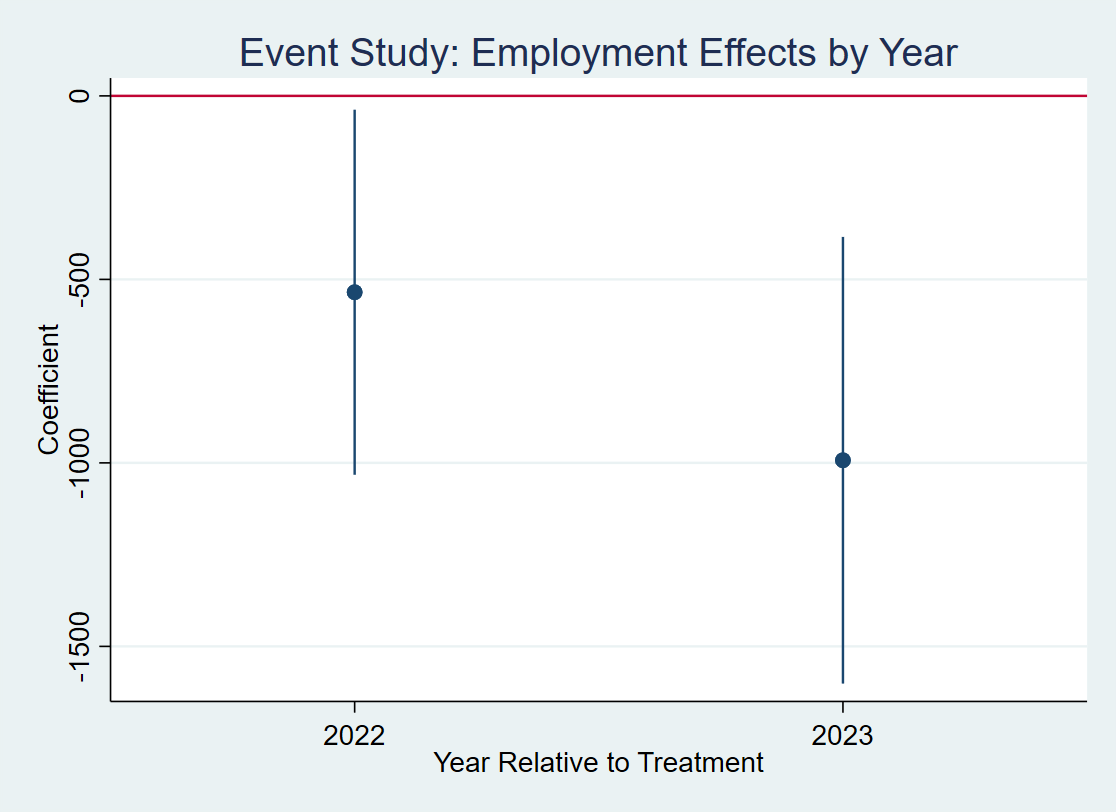
\includegraphics[width=0.85\textwidth]{fig_event_study_employment.png}
\caption{Event Study: Employment Effects Over Time}
\label{fig:event_study}
\begin{figurenotes}
\small
\item \textit{Notes:} This figure plots the event study coefficients from Table \ref{tab:event_study}, showing treatment effects for each post-treatment year relative to the omitted baseline year (2019). The negative effects appear in 2022 and grow stronger by 2023.
\end{figurenotes}
\end{figure}

\begin{figure}[H]
\centering
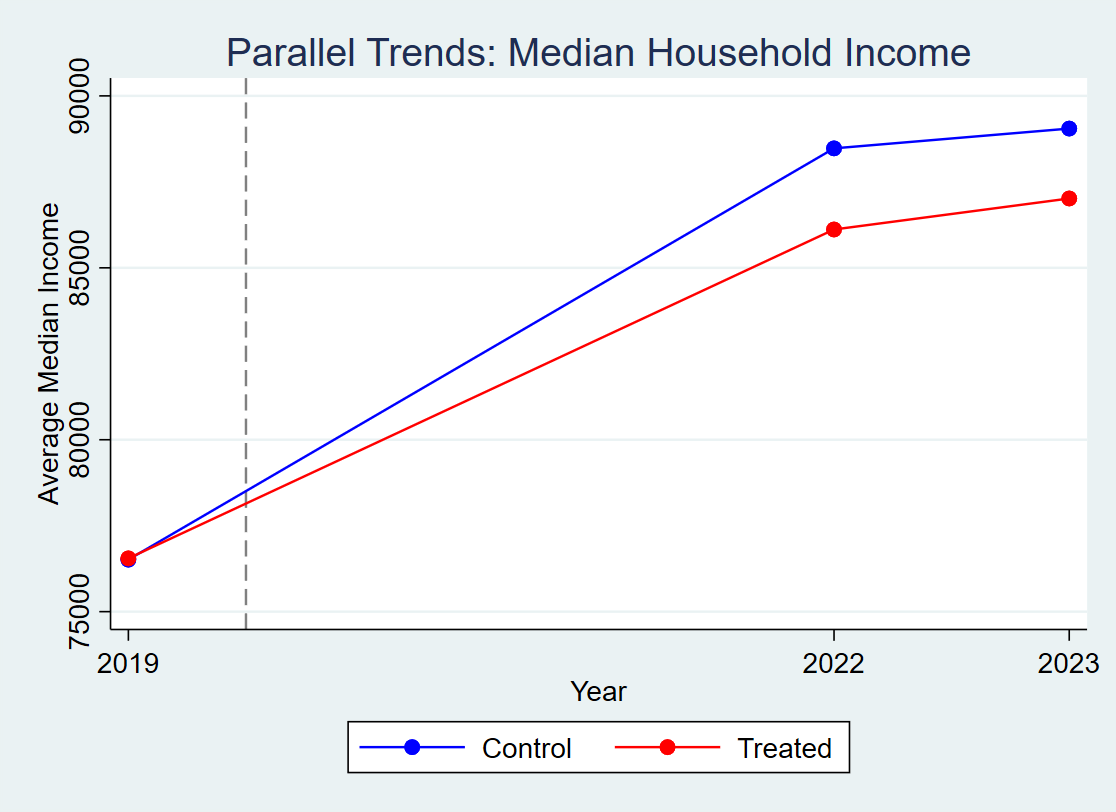
\includegraphics[width=0.85\textwidth]{fig_parallel_trends_income.png}
\caption{Parallel Trends: Median Household Income}
\label{fig:parallel_trends_income}
\begin{figurenotes}
\small
\item \textit{Notes:} This figure plots average median household income for treated and control counties over time. The vertical dashed line indicates the end of the pre-treatment period (2019). Limited to 114 counties with available income data.
\end{figurenotes}
\end{figure}

\newpage

% References
\bibliographystyle{aer}
\begin{thebibliography}{99}

\bibitem{aldashev2021}
Aldashev, A., \& Batkeyev, B. (2021). Broadband infrastructure and economic growth in rural areas. \textit{Information Economics and Policy}, 57, 100936.

\bibitem{czernich2011}
Czernich, N., Falck, O., Kretschmer, T., \& Woessmann, L. (2011). Broadband infrastructure and economic growth. \textit{The Economic Journal}, 121(552), 505-532.

\bibitem{fcc2019}
Federal Communications Commission. (2019). \textit{2019 Broadband Deployment Report}. Retrieved from https://www.fcc.gov/reports-research/reports/broadband-progress-report

\bibitem{frb2022}
Federal Reserve Bank of Richmond. (2022). The end of the digital divide? The future of broadband post-Infrastructure Investment and Jobs Act (IIJA). \textit{Regional Matters}.

\bibitem{hope2025}
Hope, J. N. A., Prah, L. F., \& Adukpo, T. K. (2025). Urban infrastructure investments and economic growth: Examining the impact of transportation, utilities, and broadband expansion in the United States. \textit{Asian Journal of Economics, Business and Accounting}, 25(5), 180-191.

\bibitem{usda2024}
U.S. Department of Agriculture. (2024). ReConnect Program. Rural Utilities Service. Retrieved from https://www.usda.gov/reconnect

\bibitem{ntia2023}
National Telecommunications and Information Administration. (2023). Broadband Equity, Access, and Deployment Program. U.S. Department of Commerce.

\end{thebibliography}

\end{document}